\documentclass{article}
\usepackage{tikz}
\usetikzlibrary{arrows.meta, decorations.markings}

\begin{document}

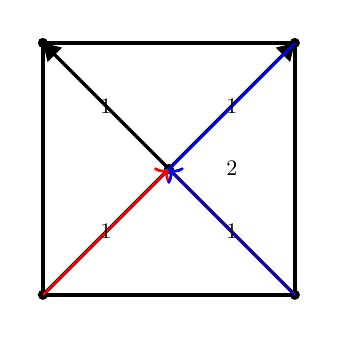
\begin{tikzpicture}[scale=0.8, transform shape]
    \draw[very thick] (0,0) -- (4,0) -- (4,4) -- (0,4) -- cycle;
    \draw[very thick, -Triangle] (0,0) -- (4,4);
    \draw[very thick, -Triangle] (4,0) -- (0,4);
    \filldraw (0,0) circle (2pt) node [anchor=north east] {};
    \filldraw (0,4) circle (2pt) node [anchor=south east] {};
    \filldraw (4,0) circle (2pt) node [anchor=north west] {};
    \filldraw (4,4) circle (2pt) node [anchor=south west] {};
    \filldraw (2,2) circle (2pt) node [anchor=south] {};
    
    % Red slice S
    \draw[thick, red, decoration={markings, mark=at position 0.5 with {\arrow[line width=1pt]{>}}}, postaction={decorate}] 
        (0,0) -- (2,2) -- (4,0);
    
    % Blue slice T
    \draw[thick, blue, decoration={markings, mark=at position 0.5 with {\arrow[line width=1pt]{>}}}, postaction={decorate}] 
        (4,0) -- (2,2) -- (4,4);
    
    % Labels for edges
    \node at (1,3) {$1$};
    \node at (3,1) {$1$};
    \node at (3,3) {$1$};
    \node at (1,1) {$1$};
    \node at (3,2) {$2$};
\end{tikzpicture}

\textit{Two adjacent, troublesome slices}: A 4-matching on \(W_5\) containing two full-index troublesome slices, \(S\) (in \textcolor{red}{red}) and \(T\) (in \textcolor{blue}{blue}), that are somewhat, but not almost disjoint. Notice that our algorithm can choose either the outer edge of \(S\) or the outer edge of \(T\), but not both.